\chapter{Literature Review}
 In this chapter, we review the foundations and advanced algorithms for shortest path calculations, including preprocessing techniques. The section spans classical algorithms, advanced algorithms and recent advances in graph-optimization.
\section{Classical shortest path algorithms}
	\subsection{Breadth-first Search}
		\subsubsection{Introduction}
		Breadth-first search is a graph traversal algorithms invented by Konrad Zuse in 1945, that can also be used to find the shortest path from a source vertex to a destination vertex in an unweighted graph.
		
		\subsubsection{Algorithm}
			\begin{enumerate}
				\item Mark all vertices as unvisited.
				\item Assign $distance[u] = \infty$ for all vertices except the source vertex $s$, where $distance[s] = 0$.
				\item Use a queue to track vertices to explore. Start with the source vertex $s$.
				\item Dequeue a vertex $u$.
				\item For each neighbour $v$ of $u$, If $v$ is unvisited (i.e., $distance[v]=\infty$):
					\begin{itemize}
						\item Set $distance[v] = distance[u] + 1$.
						\item Mark $v$ as visited.
						\item Enqueue $v$.
					\end{itemize}
				\item The algorithm ends when the queue is empty. Unreachable vertices retain $distance = \infty$.
			\end{enumerate}
			This algorithm is mathematically predisposed to find the shortest path from a source vertex $s$ to every other vertex in the graph (see\textbf{ Appendix \ref{appendix:bfs:correctness}} for a formal proof).
		
		\subsubsection{Complexity}
			When finding the shortest path between a pair of vertices in a graph, the worst-case time complexity for the BFS algorithm is $O(V)$ for queue operations + $O(E)$ for edge processing, netting a worst-case time complexity of $O(V + E)$ (see \textbf{Appendix \ref{appendix:bfs:complexity}} for a formal proof). \\ \\
			The space complexity for BFS is $O(V)$ since we use a queue to store the vertices yet to be explored.
		
		\subsubsection{Pros and Cons}
			\begin{itemize}
				\item The algorithm is simple and efficient for unweighted graphs.
				\item BFS works well for large, sparse graphs.
				\item BFS fails for shortest-path problems in weighted graphs, which are more useful when modelling real world scenarios.
			\end{itemize}
	\subsection{Bellman-ford Algorithm}
		\subsubsection{Introduction}
			The Bellman–Ford algorithm is a shortest-path algorithm that utilizes dynamic programming to compute shortest paths from a single source vertex to all of the other vertices in a weighted, directed graph. It was first published by Richard Bellman (1958) and Lester Ford Jr. (1956), hence its name.
		\subsubsection{Algorithm}
			\begin{enumerate}
				\item Create an array $distance$ of size $V$ to store the shortest path distances.
				\item Assign $distance[u] = \infty$ for all vertices except the source vertex $s$, where $distance[s] = 0$.
				\item Repeat $V - 1$ times:
					\begin{itemize}
						\item For each edge $(u,v) \in E$, if $distance[u] + w(u,v) < distance[v]$ update $distance[v]=distance[u]+w(u,v)$.
					\end{itemize}
				\item Now to detect a negative cycle, for each edge $(u,v) \in E$, if $distance[u] + w(u,v) < distance[v]$, report that a negative-weight cycle exists.
				\item If no negative-weight cycle is detected, Return the $distance$ array as the shortest path distances.
			\end{enumerate}
			Refer to \textbf{Appendix \ref{appendix:bellford:correctness}} for a formal proof of correctness of this algorithm.
		\subsubsection{Complexity}
			When finding the shortest path from a source vertex to every other vertex in a graph, the worst-case time complexity for the Bellman-Ford algorithm is $O(V \cdot E)$ (see \textbf{Appendix \ref{appendix:bellford:complexity}} for a formal proof). \\ \\
			The space complexity for Bellman-Ford is $O(V)$ since we use an array of size $V$ to store all the shortest-path distances.
		\subsubsection{Pros and Cons}
			\begin{itemize}
				\item Suitable for applications requiring negative weight handling, in which case it can detect the existence of a negative cycle.
				\item The Bellman-Ford algorithm is more complex than Dijkstra's algorithm.
				\item Much slower compared to Dijkstra's algorithm.
			\end{itemize}
	\subsection{Dijkstra's Algorithm}
		\subsubsection{Introduction}
			Dijkstra's algorithm is a greedy algorithm used to find the shortest paths from a single source vertex to all other vertices in a weighted graph with non-negative edge weights. It was conceived by computer scientist Edsger W. Dijkstra in 1956 and published three years later.
		\subsubsection{Algorithm}
		\begin{enumerate}
			\item Create an array $distance$ of size $V$ to store the shortest path distances and a priority queue $Q$ containing all vertices, prioritized by $distance$.
			\item Assign $distance[u] = \infty$ for all vertices except the source vertex $s$, where $distance[s] = 0$.
			\item While $Q$ is not empty:
				\begin{itemize}
					\item Extract the vertex u u with the smallest distance distance from $Q$.
					\item For each neighbor $v$ of $u$, if $distance[u] + w(u,v) < distance[v]$: update $distance[v]=distance[u]+w(u,v)$ and the priority of $v$ in $Q$.
				\end{itemize}
			\item The algorithm ends when $Q$ is empty. The distance distance array contains the shortest path distances from $s$ to all other vertices.
		\end{enumerate}
			Refer to \textbf{Appendix \ref{appendix:dijkstra:correctness}} for a formal proof of correctness of this algorithm.
		\subsubsection{Complexity}
			When finding the shortest path from a source vertex to every other vertex in a graph, the worst-case time complexity for the Dijkstra's algorithm is $O((V+E)\log{V})$ using a binary heap or $O(V\log{V}+E)$ using a Fibonacci heap. (see \textbf{Appendix \ref{appendix:dijkstra:complexity}} for a formal proof). \\ \\
			The space complexity for Dijkstra's is $O(V)$ since we use an array of size $V$ to store all the shortest-path distances.
		\subsubsection{Pros and Cons}
		\begin{itemize}
			\item Can cover a large area of a graph, which is useful when there are multiple target nodes.
			\item Can't calculate the shortest paths correctly if the graph has negative weights.
			\item Has linearithmetic complexity when implemented using a priority queue.
		\end{itemize}

\section{Advanced shortest path algorithms}
	\subsection{A* Search Algorithm}
		\subsubsection{Introduction}
			A* search is a heuristic-based algorithm used to find the shortest path from a start node to a goal node in a weighted graph. It combines the strengths of Dijkstra's algorithm (guaranteed shortest path) and greedy best-first search (efficient exploration using heuristics). It was first published by Peter Hart, Nils Nilsson, and Bertram Raphael at Stanford Research Institute in 1968.
		\subsubsection{Algorithm}
			\begin{enumerate}
				\item Create a priority queue $Q$ to store nodes to explore, prioritized by $f(v)=g(v)+h(v)$, where
					\begin{itemize}
						\item $g(v)$: Cost of the shortest path from $s$ to $v$ found so far.
						\item $h(v)$: Heuristic estimate of the cost from $v$ to $t$.
					\end{itemize}
				\item Set $g(s)=0$ and $f(s)=h(s)$.
				\item Insert $s$ into $Q$.
				\item Create a set $visited$ to track visited nodes
				\item While $Q$ is not empty:
					\begin{enumerate}
						\item Extract the node $u$ with the smallest $f(u)$ from $Q$.
						\item If $u=t$, return the path from $s$ to $t$.
						\item Mark $u$ as visited.
						\item For each neighbor $v$ of $u$, if $v$ is not visited:
							\begin{itemize}
								\item Compute $g_{tentative} = g(u) + w(u,v)$.
								\item If $g_{tentative} < g(v)$ or $v$ is not in $Q$:
									\begin{itemize}
										\item Update $g(v)=g_{tentative}$.
										\item Update $f(v)=g(v)+h(v)$.
										\item Insert $v$ into $Q$ (or update its priority if already in $Q$).
									\end{itemize}
							\end{itemize}
					\end{enumerate}
				\item If $Q$ becomes empty and the goal $t$ has not been reached, no path exists.
			\end{enumerate}
			A* search is correct if the heuristic $h(v)$ is admissible (never overestimates the true cost to the goal) and consistent (satisfies the triangle inequality: $h(u) \leq w(u,v)+h(v)$ for all edges $(u,v))$. For a formal proof of correctness, refer to \textbf{Appendix \ref{appendix:astar:correctness}}.
		\subsubsection{Complexity}
		Since A* Search is basically an 'informed' version of Dijkstra's algorithm, the space complexity for A* search is the same as for Dijkstra's, which is $O(V)$.
		The time complexity, however, depends on the heuristic function and is equal to Dijsktra's when the heuristic $h(v) = 0$.
		\subsubsection{Pros and Cons}
			\begin{itemize}
				\item Compared to uninformed search algorithms, A* explores significantly fewer nodes leading to faster search times. 
				\item By maintaining a priority queue, A* only needs to store a limited number of nodes in memory, making it suitable for large search spaces.
				\item Performance heavily depends on the quality of the heuristic function. Thus, A* search is not ideal when a good heuristic cannot be easily defined or when heuristic calculations are complicated.
			\end{itemize}
	\subsection{Bidirectional Search}
		\subsubsection{Introduction}
		\subsubsection{Algorithm}
		\subsubsection{Complexity}
		\subsubsection{Pros and Cons}
\section{Preprocessing techniques}
\subsection{Contraction Hierarchies}
\subsection{ALT Algorithm}
\subsection{Hub Labeling}

Refer figure \ref{fig:label}.

\section{Summary of Findings}
%\begin{figure}[htb]
%\centering
%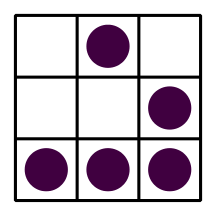
\includegraphics[scale=0.3]{./glider} % e.g. insert ./image for image.png in the working directory, adjust scale as necessary
%\caption{Caption here}
%\label{fig:label} % insert suitable label, this is used to refer to a fig from within the text as shown above
%\end{figure}

\section{Gaps in current approaches}
	\begin{itemize}
		\item Limited scalability in dynamic graphs.
		\item Lack of flexibility for user preferences.
		\item High preprocessing overhead in large graphs.
	\end{itemize}

